\chapter{Results and analysis}

We performed classification with four different classifiers on four different datasets. In each dataset-classifier combination we measured classification accuracy when applying four different feature selection (FS) methods. The aim is to investigate the impact of feature selection, and the interaction between different classifiers and FS-methods. To build a basis for comparisons, classification accuracy was measured without FS too.

\section{Variation among factors of experiments}
\label{Variation_among_factors}

Before analyzing the results we consider potential interactions between different factors involved in the experiment, these are:

\begin{enumerate}
  \item Datasets
  \item Machine Learning classifiers
  \item Feature selection methods
\end{enumerate}

Having four of each factor, there are 64 distinct combinations. We are particular interested in two of the interactions, Datasets:FS-methods and Classifiers:FS-methods.

\subsection{Datasets with larger dimensionality achieves better classification accuracy}

Studying the interaction between datasets and FS-methods, we regarded these factors as independent variables (IVs). Each IV combination is represented by four values, the best accuracy achieved with current FS-method by each of the four classifiers.

Two-way analysis of variance (ANOVA) is performed on the IVs. The results are found in \ref{table:anova_values_data} and suggests three conclusions:

% ANOVA computations, dataset-fs
\begin{table}[ht]
  \begin{center}
  \begin{tabular}{l|r|r|r|r|r|r|}
  \cline{2-7}
  & $RSS$ & $df$ & $F$ & $P(>F)$ & $\eta^2$ & $\omega^2$ \\ \cline{1-7}
  \multicolumn{1}{ |l| }{\textbf{Dataset}}
  & 0.7383 &  3.0 & 15.939 & 2.5241e-07 & 0.4757 & 0.4415 \\
  \cline{1-7}
  \multicolumn{1}{ |l| }{\textbf{Method}}
  & 0.0099 &  3.0 & 0.2137 & 8.8645e-01 & 0.0064 & -0.0232 \\
  \cline{1-7}
  \multicolumn{1}{ |l| }{\textbf{Dataset:Method}}
  & 0.0627 &  9.0 & 0.4514 & 8.9938e-01 & 0.0404 & -0.0486 \\
  \cline{1-7}
  \multicolumn{1}{ |l| }{\textbf{Residual}}
  & 0.7412 &  48.0 \\ \cline{1-3}
  \end{tabular}
  \caption{ANOVA values of accuracy in relation to dataset, method and the interaction of datasets and methods.}
  \label{table:anova_values_data}
  \end{center}
\end{table}


First, the significance of Dataset allows to conclude a dependency between accuracies and datasets is present. This is to be expected because different datasets provide varying basis for prediction. However, as all accuracies used in the test was obtained by feature selection this test gives no information on whether the correlation lies among the datasets themselves of the application of feature selection.

Secondly, absent significance of Method conclude we can not reject that there is no correlation between FS-method and accuracy.

Thirdly, no significance of Dataset:Method indicates we can not reliably conclude that the interaction between datasets and methods has a correlation with achieved accuracy.

Visualizing the values used in the ANOVA test we can spot the found correlation between datasets and accuracy \ref{fig:comp_acc_datasets}. The correlation appears positive in respect to number of attributes suggesting either feature selection has a larger impact on classification accuracy when data has a higher dimensionality or higher dimensioned datasets on their own lead to better accuracy.

\begin{figure*}[ht]
  \centering
    \begin{subfigure}[b]{0.475\textwidth}
        \centering
        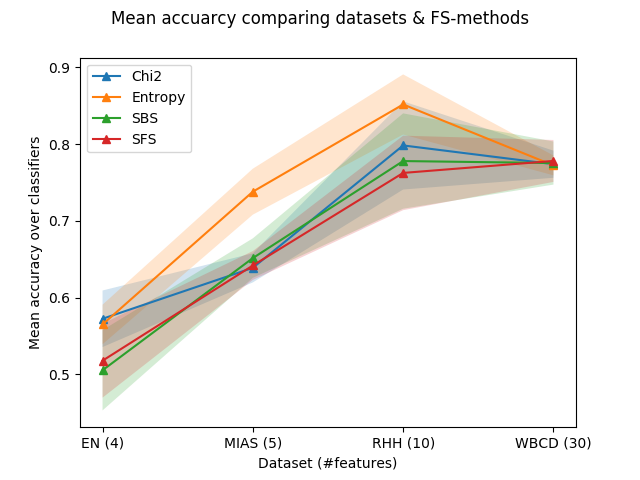
\includegraphics[width=\textwidth]{../plots_with_std_fill/comp_acc_datasets.png}
        \caption[]%
        {{\small Datasets and accuracy displays evident correlation independently of applied FS method.}}
        \label{fig:comp_acc_datasets}
    \end{subfigure}
  \hfill
    \begin{subfigure}[b]{0.475\textwidth}
        \centering
        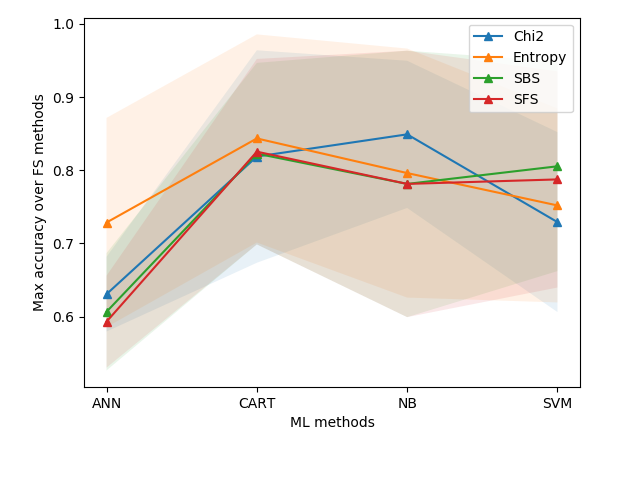
\includegraphics[width=\textwidth]{../plots_with_std_fill/comp_classif_datasets.png}
        \caption[]%
        {{\small Some correlation between different classifiers and FS-methods is evident.}}
        \label{fig:comp_classif_datasets}
    \end{subfigure}
  \caption[]
  {\small Good caption goes here.}
  \label{fig:anova_plots}
\end{figure*}


\subsection{FS-methods are classifier dependent}
\label{sec:fs_methods_classifiers}

To investigate the effect of feature selection on different classifiers two-way ANOVA we performed two-way ANOVA. The values constitutes of each accuracy achieved of all distinct classifier and FS-method on all datasets.

First we are interested in the characteristics of the interaction, secondly if these characteristics are significant.

First, we compare classification accuracy between different classifiers and FS-methods by plotting the mean accuracy over all datasets for each classifier-FS combination, \ref{fig:comp_classif_datasets}. The plot shows no clear correlation suggesting behavior of such combinations are independent.

Secondly, to conclude interaction between classifiers and FS-methods is independent we performed two-way ANOVA. The results can be viewed in table \ref{table:anova_values_classif}. Looking at the P-value for accuracy in relation to the interaction between Classifier:Method we can conclude that these interactions are independent with a confidence level of 95\%.

\begin{table}[ht]
  \begin{center}
  \begin{tabular}{l|r|r|r|r|r|r|}
  \cline{2-7}
  & $RSS$ & $df$ & $F$ & $P(>F)$ & $\eta^2$ & $\omega^2$ \\ \cline{1-7}
  \multicolumn{1}{ |l| }{\textbf{Classifier}}
  & 0.3336 &  3.0 & 16.491 & 1.6860e-07 & 0.2149 & 0.2010 \\
  \cline{1-7}
  \multicolumn{1}{ |l| }{\textbf{Method}}
  & 0.7383 &  3.0 & 36.495 & 1.9503e-12 & 0.4757 & 0.4607 \\
  \cline{1-7}
  \multicolumn{1}{ |l| }{\textbf{Classifier*Method}}
  & 0.1565 &  9.0 & 2.5783 & 1.6490e-02 & 0.1008 & 0.0614 \\
  \cline{1-7}
  \multicolumn{1}{ |l| }{\textbf{Residual}}
  & 0.3237 &  48.0 \\ \cline{1-3}
  \end{tabular}
  \caption{Set caption.}
  \label{table:anova_values_classif}
  \end{center}
\end{table}


These results suggests one has to carefully select the classifier and FS-method to achieve optimal results.


\section{Classification improvements}

After performing classification with and without FS-methods, all results of each classifier was collected. Results are presented in tables for ANN \ref{table:ANN}, CART \ref{table:CART}, NB \ref{table:NB} and SVM \ref{table:SVM} where the highest achieved accuracy is highlighted in bold format. From this we can conclude that classification accuracy is equal or improved for all classifiers on all datasets tested in our scope by use of \textit{some} feature selection method. The only exception is the Mias dataset with Decision tree \ref{table:CART}, it performed worse with feature selection.

However, majority of the classifiers has some FS-method that achieved lower accuracy compared to full dataset. Again this is viewed in tables \ref{table:ANN}, \ref{table:CART}, \ref{table:NB} and \ref{table:SVM}. In 11 of 16 instances at least one FS-method performed worse. This is in line with our findings that FS-method is classifier dependent suggesting one have to select the combination of classifier and FS-method with care.

% --- Tables ---
\begin{table}[h]
  \centering
  \begin{tabular}{|l|l|l|l|l|l}
\cline{1-5}
        \textbf{ANN} & MIAS              & EN                & RHH               & WBCD      &         \\
\cline{1-5}
Chi2    & 0.58 & 0.59 & 0.64 & 0.71 \\
Entropy & 0.56 & \textbf{0.84} & \textbf{0.90} & 0.62 \\
SBS     & 0.54 & 0.55 & 0.59 & \textbf{0.74} \\
SFS     & \textbf{0.59} & 0.51 & 0.59 & 0.68 \\
Full    & 0.57 & 0.68 & 0.60 & 0.53 \\
\cline{1-5}
Gain    & 0.04 & 0.24 & 0.51 & 0.41 & 1.2 \\
\cline{1-5}
\end{tabular}

  \caption[]%
  {{\small Classification accuracy achieved by ANN. Accuracy improved on all datasets by the use of some feature selection method. Rows represent feature selection method, columns represent dataset, bold font indicates the highest value.}}
  \label{table:ANN}
\end{table}

\begin{table}[h]
  \centering
  \begin{tabular}{|l|l|l|l|l|l}
\cline{1-5}
        \textbf{CART} & MIAS              & EN                & RHH               & WBCD      &         \\
\cline{1-5}
Chi2    & 0.70           & 0.69           & 0.90           & \textbf{0.97}  &         \\
Entropy & 0.53           & \textbf{0.83}  & 0.91           & 0.96           &         \\
SBS     & 0.63           & 0.67           & 0.91           & 0.95           &         \\
SFS     & 0.67           & 0.67           & \textbf{0.92}  & \textbf{0.97}  &         \\
Full    & \textbf{0.77}  & 0.69           & 0.90           & 0.94           &         \\
\cline{1-5}
\cline{1-5}
Gain    & -0.09           & 0.21           & 0.03           & 0.03           & 0.18 \\
\cline{1-5}
\end{tabular}
 \\
  \caption[]%
  {{\small All datasets except MIAS benefited in classification accuracy from feature selection using CART Decision Tree classifier. Rows represent feature selection method, columns represent dataset, bold font indicates the highest value.}}
  \label{table:CART}
\end{table}

\begin{table}[h]
  \centering
  \begin{tabular}{|l|l|l|l|l|l}
\cline{1-5}
        & MIAS              & EN                & RHH               & WBCD      &         \\
\cline{1-5}
Chi2    & \textbf{0.77}  & \textbf{0.74}  & \textbf{0.94}  & 0.96           &         \\
Entropy & \textbf{0.77}  & 0.55           & 0.91           & 0.97           &         \\
SBS     & 0.43           & 0.71           & 0.91           & \textbf{0.97}  &         \\
SFS     & 0.43           & 0.71           & 0.91           & \textbf{0.97}  &         \\
Full    & \textbf{0.77}  & 0.66           & \textbf{0.94}  & 0.96           &         \\
\cline{1-5}
\cline{1-5}
Gain    & 0                 & 0.12           & 0                 & 0.01           & 0.14 \\
\cline{1-5}
\end{tabular}
 \\
  \caption[]%
  {{\small Na\"ive Bayes sees improvement or equivalent accuracy by feature selection on every dataset. Rows represent feature selection method, columns represent dataset, bold font indicates the highest value.}}
  \label{table:NB}
\end{table}

\begin{table}[h]
  \centering
  \begin{tabular}{|l|l|l|l|l|l}
\cline{1-5}
        \textbf{SVM} & MIAS              & EN                & RHH               & WBCD      &         \\
\cline{1-5}
Chi2    & \textbf{0.57}  & 0.73           & 0.90           & 0.63           &         \\
Entropy & 0.33           & \textbf{0.83}  & \textbf{0.91}  & 0.63           &         \\
SBS     & 0.53           & 0.68           & 0.88           & \textbf{0.93}  &         \\
SFS     & 0.53           & 0.68           & 0.88           & \textbf{0.93}  &         \\
Full    & \textbf{0.57}  & 0.73           & 0.90           & 0.61           &         \\
\cline{1-5}
\cline{1-5}
Gain    & 0                 & 0.14           & 0.02           & 0.51           & 0.68 \\
\cline{1-5}
\end{tabular}
 \\
  \caption[]%
  {{\small Classification accuracy achieved by SVM. Accuracy was improved or equivalent on every dataset with use of feature selection. Rows represent feature selection method, columns represent dataset, bold font indicates the highest value.}}
  \label{table:SVM}
\end{table}
% ---/Tables ---

\subsection{Improvement is significant}

To ensure the suggestion that application of some FS-method improves classification accuracy t-test was performed. Regarding the accuracies achieved without feature selection as one distribution and best accuracies achieved with feature selection as the other.

Performing the t-test the resulting P-value was 0.077. This allows us to reject the null hypothesis that the distributions are equal with a confidence level of 90\%. Thus proving improvement of classification accuracy by feature selection is statistically significant.

\subsection{Differences among classifiers}

As addressed in section \ref{Variation_among_factors} classifiers behave differently depending on FS-method and datasets.
In order to compare classification improvement among different FS-methods and datasets \textbf{Gain} is computed. Gain measures the improvement of FS as the ratio between best achieved FS accuracy and full dataset accuracy. The accumulated gain for each classifier is presented in \ref{table:gain_comparison}. Below these results and differences are analyzed in further detail with respect to each classifier.

\begin{table}[hp]
  \begin{tabular}{|l|l|l|l|}
\hline
Ranking  & Classifier                & Accumulated gain  & Average gain\\
\hline
1        & Artificial Neural Network & 1.34   & 34\%        \\
2        & Support Vector Machine    & 0.68  & 17\%       \\
3        & Decision Tree             & 0.18   & 5\%         \\
4        & Naïve Bayes               & 0.14   & 4\%         \\
\hline
\end{tabular}

  \caption[]%
  {{\small Ranking of which classifiers gained most accuracy when comparing feature selection to full dataset.}}
  \label{table:gain_comparison}
\end{table}

\subsubsection{Artificial Neural Network}

Looking at the table \ref{table:gain_comparison} the accumulated gain was 1.34 which was the highest among all classifiers. However, ANN consistently performs the worst of all classifiers in terms of accuracy. The ANN also provides the least consistent results with strong fluctuations in the results and wide standard deviation margins. Such fluctuations may suggest issues regarding convergence. These characteristics are evident in plot \ref{fig:WBCD_chi2} showcasing the accuracy by each FS-method as a function of number of attributes..

\subsubsection{Support Vector Machine}

The SVM behaves very differently in respect to each dataset. Improvements are seen with a larger subset of attributes in the EN and MIAS dataset as seen in \ref{fig:EN_chi2} and \ref{fig:MIAS_sfs}. A negative trend on accuracy is observed on the WBCD datasets which might indicate an issue with dimensionality. In \ref{fig:RHH_sbs} an improved accuracy is evident with maximal accuracy achieved on a subset suggesting a positive effect of feature selection.

\subsubsection{Decision Tree}

The decision tree shows consistent performance generally increasing performance with an increased amount of features. Although in cases like plot \ref{fig:WBCD_chi2} and \ref{fig:MIAS_sbs} best accuracy is achieved with a subset of features displaying evident benefits of feature selection.

\subsubsection{Naïve Bayes}

Naive Bayes had the least accumulated gain from feature selection as seen in table \ref{table:gain_comparison}. The largest improvement was seen in plot \ref{fig:EN_chi2} using 2 of 4 available attributes. In plots \ref{fig:WBCD_entropy} and \ref{fig:RHH_entropy} the accuracy sees little to no improvement when increasing the number of attributes.

\subsection{Combined plots of mean accuracy}
\begin{figure*}[htp]
  \centering
  \begin{subfigure}[b]{0.475\textwidth}
      \centering
      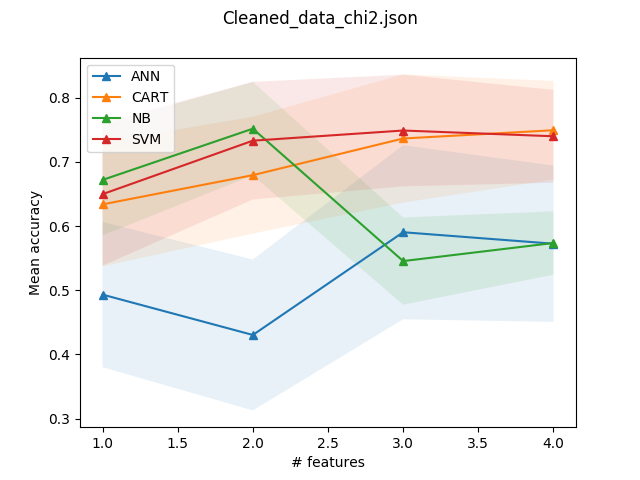
\includegraphics[width=\textwidth]{../plots_with_std_fill/Cleaned_data_chi2_combined.png}
      \caption[]%
      {{\small}}
      \label{fig:EN_chi2}
  \end{subfigure}
  \hfill
  \begin{subfigure}[b]{0.475\textwidth}
      \centering
      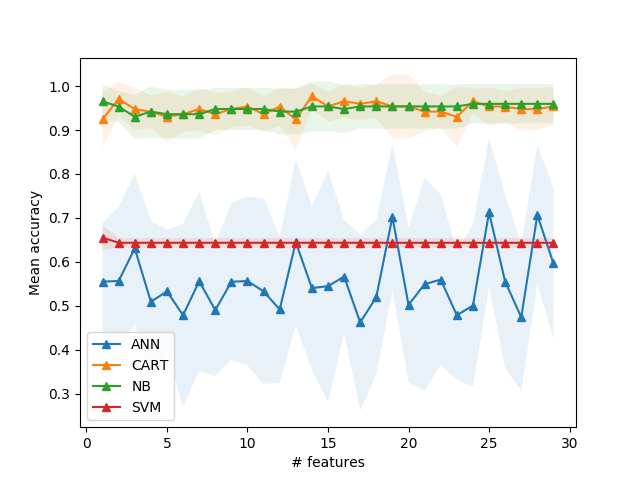
\includegraphics[width=\textwidth]{../plots_with_std_fill/data_FNA_chi2_combined.png}
      \caption[]%
      {{\small}}
      \label{fig:WBCD_chi2}
  \end{subfigure}
  \vskip\baselineskip
  \begin{subfigure}[b]{0.475\textwidth}
      \centering
      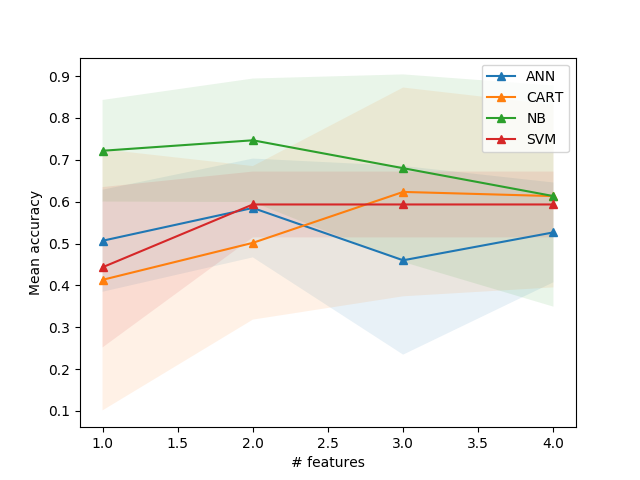
\includegraphics[width=\textwidth]{../plots_with_std_fill/Data_mias_chi2_combined.png}
      \caption[]%
      {{\small}}
      \label{fig:MIAS_chi2}
  \end{subfigure}
  \quad
  \begin{subfigure}[b]{0.475\textwidth}
      \centering
      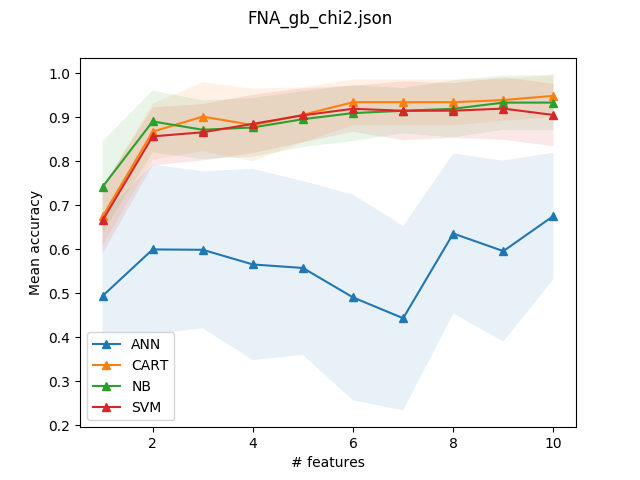
\includegraphics[width=\textwidth]{../plots_with_std_fill/FNA_gb_chi2_combined.png}
      \caption[]%
      {{\small}}
      \label{fig:RHH_chi2}
  \end{subfigure}
  \caption[]
  {\small a: Dataset EN using Chi2, b: Dataset WBCD using Chi2, c:  Dataset MIAS using Chi2, d: Dataset RHH using Chi2.  Combined plots of all datasets comparing each classifier when using chi2 for feature selection.}
  \label{fig:plots_chi2}
\end{figure*}

\begin{figure*}[htp]
  \centering
  \begin{subfigure}[b]{0.475\textwidth}
      \centering
      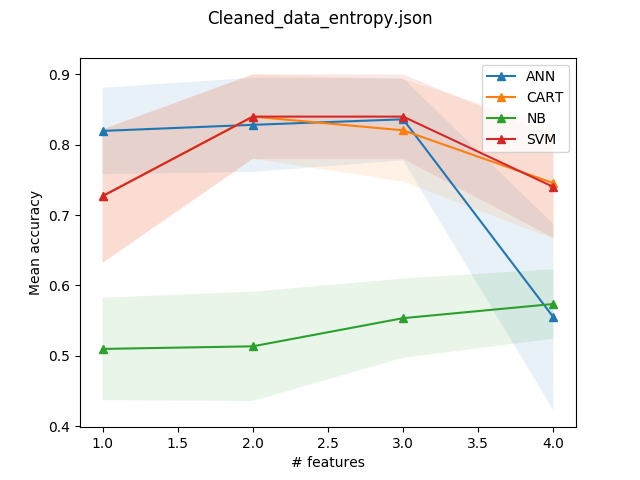
\includegraphics[width=\textwidth]{../plots_with_std_fill/Cleaned_data_entropy_combined.png}
      \caption[Network2]%
      {{\small }}
      \label{fig:EN_entropy}
  \end{subfigure}
  \hfill
  \begin{subfigure}[b]{0.475\textwidth}
      \centering
      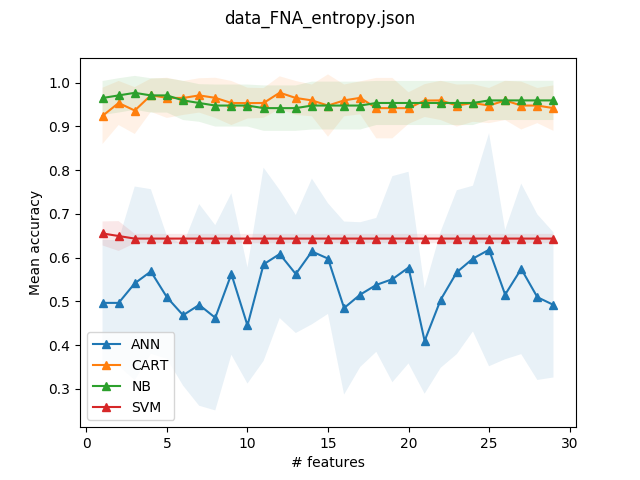
\includegraphics[width=\textwidth]{../plots_with_std_fill/data_FNA_entropy_combined.png}
      \caption[]%
      {{\small}}
      \label{fig:WBCD_entropy}
  \end{subfigure}
  \vskip\baselineskip
  \begin{subfigure}[b]{0.475\textwidth}
      \centering
      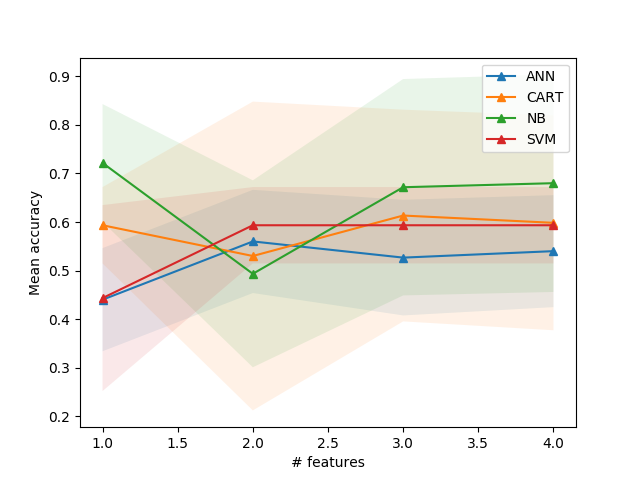
\includegraphics[width=\textwidth]{../plots_with_std_fill/Data_mias_entropy_combined.png}
      \caption[]%
      {{\small }}
      \label{fig:MIAS_entropy}
  \end{subfigure}
  \quad
  \begin{subfigure}[b]{0.475\textwidth}
      \centering
      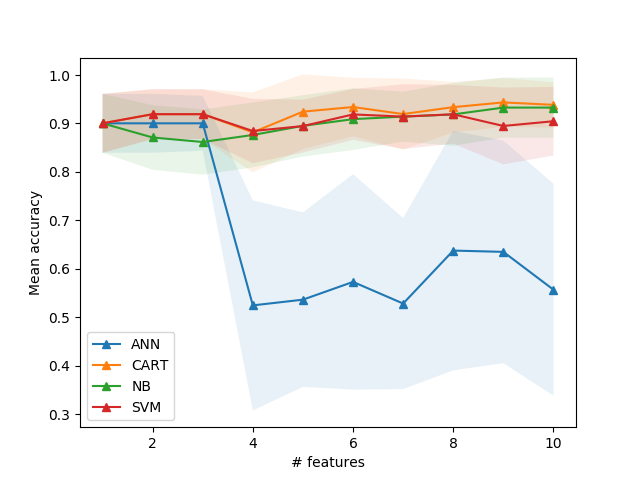
\includegraphics[width=\textwidth]{../plots_with_std_fill/FNA_gb_entropy_combined.png}
      \caption[]%
      {{\small }}
      \label{fig:RHH_entropy}
  \end{subfigure}
  \caption[]
  {{\small a: Dataset EN using Entropy, b: Dataset WBCD using Entropy, c: Dataset MIAS using Entropy, d: Dataset RHH using Entropy. Combined plots of all datasets comparing each classifier when using Entropy for feature selection.}}
  \label{fig:plots_entropy}
\end{figure*}

\begin{figure*}[htp]
  \centering
  \begin{subfigure}[b]{0.475\textwidth}
      \centering
      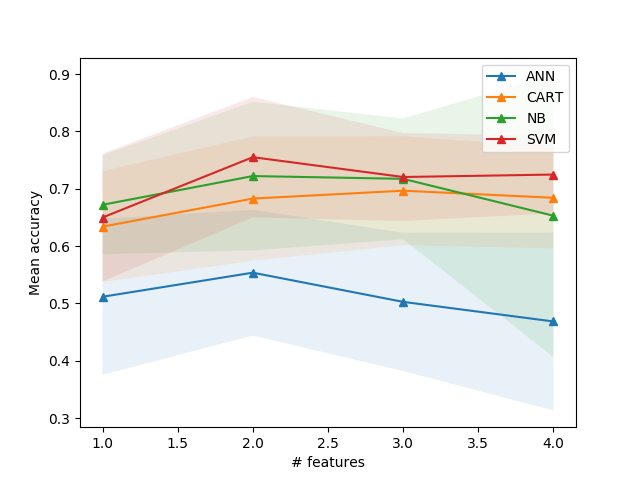
\includegraphics[width=\textwidth]{../plots_with_std_fill/Cleaned_data_sb_combined.png}
      \caption[]%
      {{\small}}
      \label{fig:EN_sbs}
  \end{subfigure}
  \hfill
  \begin{subfigure}[b]{0.475\textwidth}
      \centering
      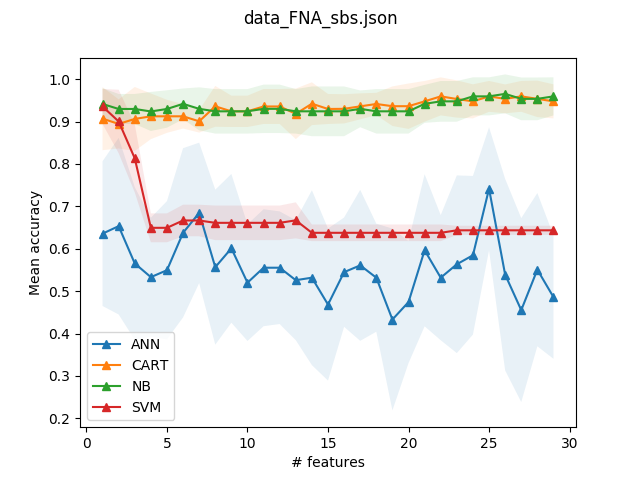
\includegraphics[width=\textwidth]{../plots_with_std_fill/data_FNA_sb_combined.png}
      \caption[]%
      {{\small}}
      \label{fig:WBCD_sbs}
  \end{subfigure}
  \vskip\baselineskip
  \begin{subfigure}[b]{0.475\textwidth}
      \centering
      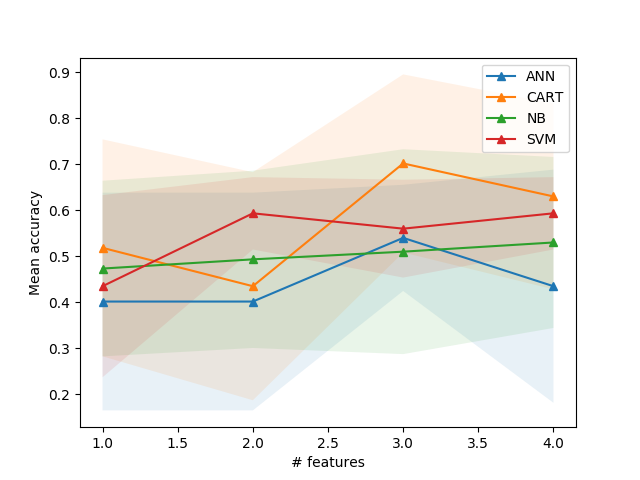
\includegraphics[width=\textwidth]{../plots_with_std_fill/Data_mias_sb_combined.png}
      \caption[]%
      {{\small}}
      \label{fig:MIAS_sbs}
  \end{subfigure}
  \quad
  \begin{subfigure}[b]{0.475\textwidth}
      \centering
      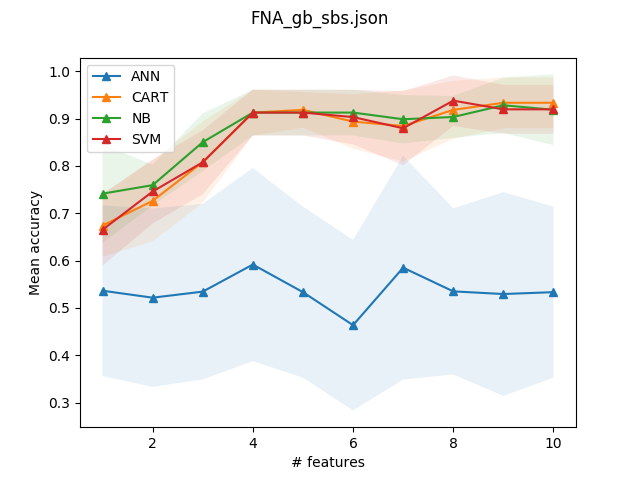
\includegraphics[width=\textwidth]{../plots_with_std_fill/FNA_gb_sb_combined.png}
      \caption[]%
      {{\small}}
      \label{fig:RHH_sbs}
  \end{subfigure}
  \caption[]
  {{\small (a) Dataset EN using SBS. (b) Dataset WBCD using SBS. (c) Dataset MIAS using SBS. (d) Dataset RHH using SBS. Combined plots of all datasets comparing each classifier when using SBS for feature selection.}}
  \label{fig:plots_sbs}
\end{figure*}

\begin{figure*}[htbp!]
  \centering
  \begin{subfigure}[b]{0.475\textwidth}
      \centering
      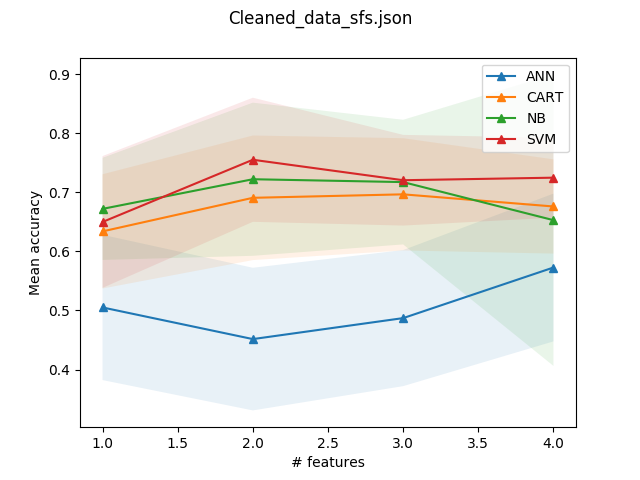
\includegraphics[width=\textwidth]{../plots_with_std_fill/Cleaned_data_sf_combined.png}
      \caption[]%
      {{\small Dataset EN using SFS}}
      \label{fig:EN_sfs}
  \end{subfigure}
  \hfill
  \begin{subfigure}[b]{0.475\textwidth}
      \centering
      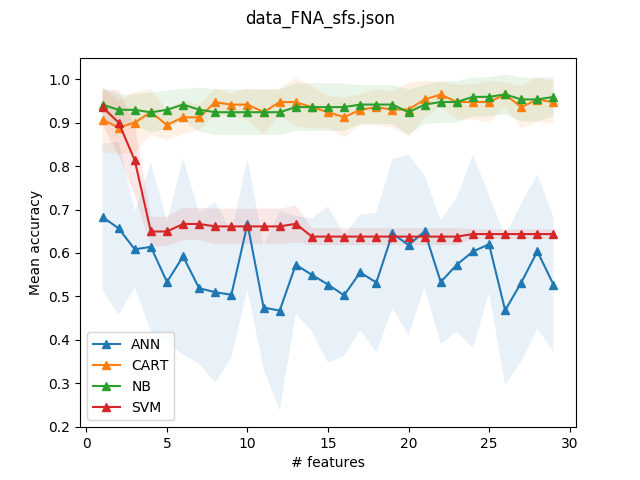
\includegraphics[width=\textwidth]{../plots_with_std_fill/data_FNA_sf_combined.png}
      \caption[]%
      {{\small Dataset WBCD using SFS}}
      \label{fig:WBCD_sfs}
  \end{subfigure}
  \vskip\baselineskip
  \begin{subfigure}[b]{0.475\textwidth}
      \centering
      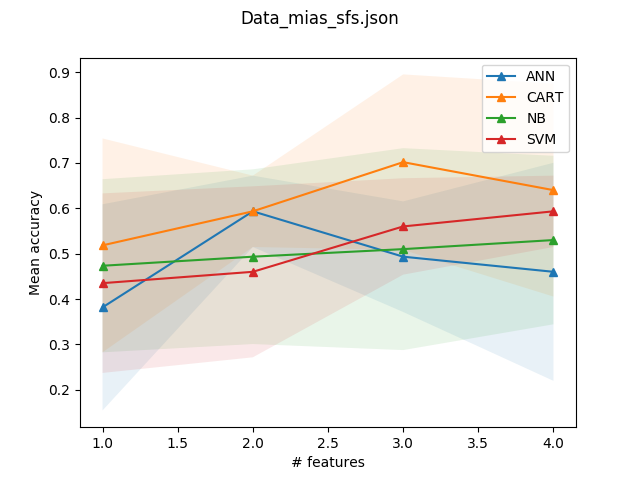
\includegraphics[width=\textwidth]{../plots_with_std_fill/Data_mias_sf_combined.png}
      \caption[]%
      {{\small Dataset MIAS using SFS}}
      \label{fig:MIAS_sfs}
  \end{subfigure}
  \quad
  \begin{subfigure}[b]{0.475\textwidth}
      \centering
      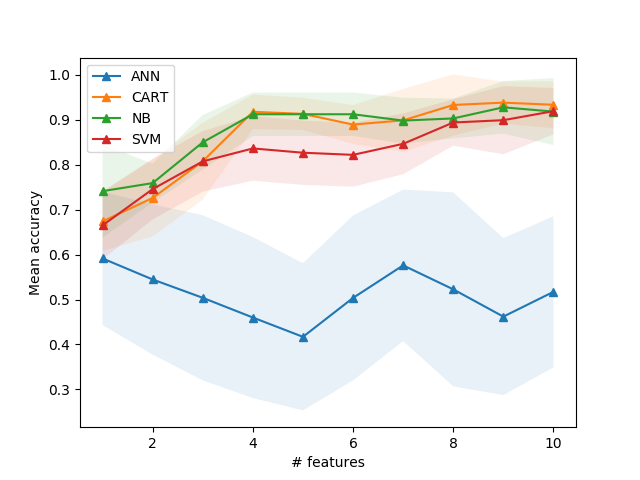
\includegraphics[width=\textwidth]{../plots_with_std_fill/FNA_gb_sf_combined.png}
      \caption[]%
      {{\small Dataset RHH using SFS}}
      \label{fig:RHH_sfs}
  \end{subfigure}
  \caption[]
  {{\small Combined plots of all datasets comparing each classifier when using SFS for feature selection.}}
  \label{fig:plots_sfs}
\end{figure*}



\section{Computation time}

\textbf{Under construction, profiling not run yet.}

Profiling the execution of running all experiments X\% of CPU-time was allocated to the Wrapper algorithms. As mentioned a finding the best possible subset of features is considered a NP-hard problem meaning a solution can not be found in polynomial time. This clearly suggest favouring filtering methods when choosing a feature selection method having limited computational resources.

\section{Source of errors}
\label{sec:source_of_errors}

There are two main factor that may risk propagate error into the results, libraries and datasets.

The libraries provide all functionality of the classifiers, filter selection methods and analysis tools. A major part of the implementation therefore constitutes of these libraries. A implementation built upon faulty methods can not provide any trustworthy results. The Scikit library \parencite{scikit-learn} is well renowned and widely used in both industry and research thus inspire confidence in its robustness. The mlxtend library is used for SBS and SFS methods and is still a open source with less coverage than Scikit \parencite{mlextend}. Still it has a active community and many release versions indicating it's well managed.

Because we use a multitude of datasets their differences may influence our results in a way that invalidates our findings. \textcite{c201416} claim that feature selection methods can only be compared on the same dataset. However our comparisons do not regard the performance of specific FS-methods but their impact at large. Also, these interactions is addressed in \ref{Variation_among_factors}.

Due to varying number of examples of the datasets where some are rather small, evaluation by kFold may infer very small test batches and lead to skewed results. The impact may be enlarged considering our classification is binary. This influence is minimized by using stratified kFold but as no check of distribution of classes in test batches was made this might be a source of error.
